\documentclass[10pt,a4paper]{article}
\usepackage[margin=2.2cm]{geometry}
\usepackage{amsmath,amssymb,booktabs,graphicx,microtype}
\usepackage[hidelinks]{hyperref}
\usepackage{caption}
\captionsetup{font=small,labelfont=bf}

\title{Mechanism-Dependent Degradation of Filtered Approximate Nearest Neighbor Indexes under Data Churn}
\author{Vladimir Asonov\\\small HSE University, Moscow, Russia}
\date{Preprint, September 2026}

\begin{document}
\maketitle

\begin{abstract}
Filtered approximate nearest neighbor (ANN) search --- vector search restricted to objects that satisfy an attribute predicate --- underlies vector databases and retrieval-augmented generation, where collections are updated continuously. Yet filtered ANN methods are evaluated on static data, and production systems schedule index maintenance by fixed constants such as ``rebuild at 20\% deleted''. We measure how three filtered ANN methods with three different maintenance mechanisms degrade under a sustained stream of deletions and insertions, tracking recall against exact filtered ground truth at every checkpoint and search work as the number of distance computations. On SIFT and on YFCC-10M with real tags, degradation is determined by the maintenance mechanism: HNSW with mark-delete keeps recall but its work per query grows as $p^{-\beta}$ with the live fraction $p$ of graph vertices ($\beta = 0.89$--$1.02$, 0.5--1.9\% error over three seeds); Filtered-DiskANN with lazy deletion loses recall, behaving like a fresh index with a shrunken candidate list $L\,p^{\alpha}$ ($\alpha = 0.69$ fitted on one run reduces held-out error from 0.019 to 0.002--0.003); a static index (UNG) rebuilt at deleted fraction $t$ delivers time-averaged recall $1 - t/2$ (within 0.004). Degradation of Filtered-DiskANN grows as the filter narrows, while the other two mechanisms are nearly insensitive to selectivity. The laws turn the choice of a maintenance threshold into an optimization problem instead of a constant. We also report reproducibility pitfalls met while driving the methods under churn.
\end{abstract}

\section{Introduction}

Almost every query to a vector database carries a filter: a tenant, access rights, availability, a time range. Filtered ANN methods --- predicate-agnostic traversal \cite{acorn}, label-aware graph construction \cite{filtereddiskann}, label-partitioned graphs \cite{ung} or post-filtered HNSW \cite{hnsw} --- are compared on collections that are built once and then queried. In operation, data are deleted and inserted all the time, deletions are usually lazy, and the index drifts away from the structure it was built with. Practitioners observe the effect: in one reported case, filtered recall of a production index fell from 89\% to 34\% and only a full rebuild helped \cite{qdrant}. Maintenance is nevertheless triggered by constants unrelated to search quality (a deleted fraction of 20\% in several systems).

Recent benchmarks add update phases at the level of database systems \cite{vecbench} or evaluate filters and dynamics separately \cite{annlib}; streaming ANN work studies updates without filters \cite{freshdiskann,bigann23}. What is missing is a trajectory-level view of \emph{filtered} search quality under churn, measured against exact filtered ground truth, and an account of \emph{why} methods degrade differently.

\paragraph{Contributions.} (1) A measurement protocol: deterministic update scenarios, exact filtered ground truth at every checkpoint, recall trajectories with tail statistics, and machine-independent work per query. (2) Measurements of three filtered ANN methods representing three maintenance mechanisms on SIFT and on YFCC-10M with real tags. (3) Three first-order laws, one per mechanism, each with a single parameter, validated on held-out runs; the mechanisms are traced to the methods' source code. (4) The dependence of degradation on filter selectivity. (5) Reproducibility pitfalls encountered when driving these methods under churn.

\section{Protocol}

\paragraph{Methods.} HNSW via hnswlib \cite{hnsw} with an external filter functor, in two deletion modes: \emph{mark-delete} (deleted vertices stay in the graph) and \emph{slot reuse} (new points overwrite deleted slots). Filtered-DiskANN \cite{filtereddiskann} (C++ branch, dynamic in-memory index) with lazy deletion, either never consolidated or consolidated every 10{,}000 deletions. UNG \cite{ung}, a static index, served between rebuilds (deleted objects are filtered out of answers, new objects are invisible) and rebuilt when the deleted fraction reaches $t$ of the live objects. ACORN \cite{acorn} was excluded from dynamic scenarios (Section~\ref{sec:pitfalls}). Each method runs in its own container through a small C++ driver that replays the same operation stream; all revisions are pinned.

\paragraph{Data and filters.} SIFT \cite{sift} (100k base vectors, 20 synthetic Zipf-distributed or k-means labels). YFCC-10M from the NeurIPS'23 filtered track \cite{bigann23,yfcc}: CLIP embeddings with real tags (a 1M prefix; 8.8 tags per object). Filters are single tags chosen deterministically by share; the queries of a tag filter are the first 300 public queries carrying that tag, preserving the correlation between content and tags. For YFCC the tag vocabulary is reduced to the queried tags plus an ``other'' label, which does not change answers for these filters.

\paragraph{Scenarios and measurements.} \emph{Steady churn}: from 100k objects, each step deletes a random live object and inserts a new one; 300k steps renew the collection three times. \emph{Category purge}: all objects of one category are deleted at once, followed by insertions. At every checkpoint we compute exact filtered top-10 neighbors of the live collection and report recall@10 (mean, 5th percentile, share of queries below 0.9) and the number of distance computations per query. Methods are compared at a common operating point: recall@10 $\geq 0.98$ on a fresh index both without a filter and with the widest filter (hnswlib $ef=128$, UNG $L=100$, Filtered-DiskANN $L=100$ on YFCC; $ef=64$, $L=100$, $L=300$ on SIFT). The testbed is a single 8-vCPU, 16~GB virtual machine (the normalized streaming-track configuration); runs are sequential.

\section{Results}

\begin{figure}[t]
\centering
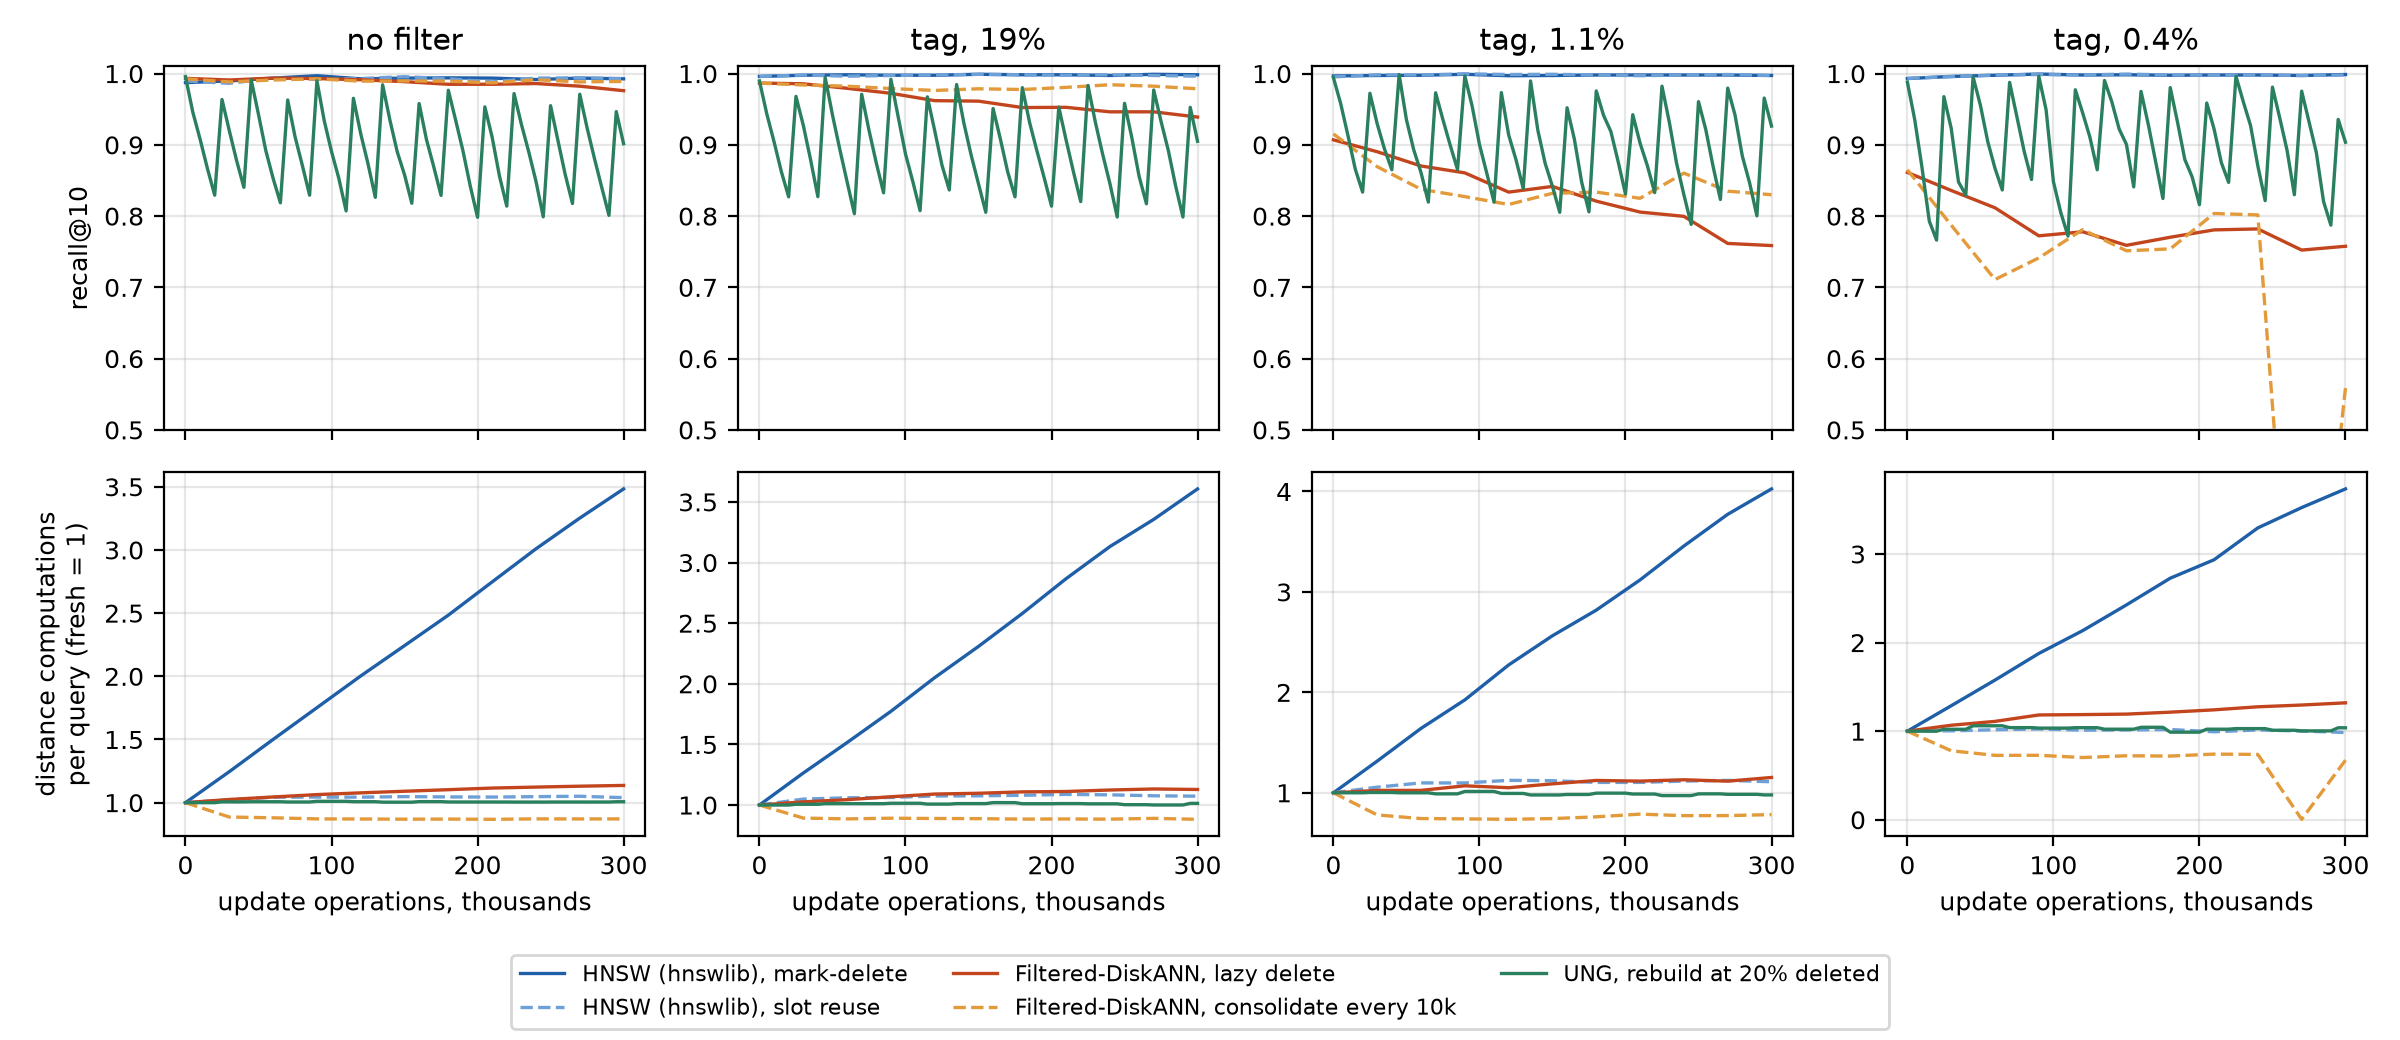
\includegraphics[width=\linewidth]{figures/fig_mechanisms.png}
\caption{YFCC-10M, steady churn renewing the collection three times. Top: recall@10; bottom: distance computations per query relative to the fresh index. Columns: no filter and tags covering 19\%, 1.1\% and 0.4\% of the collection. One seed shown; Table~\ref{tab:main} gives ranges over three.}
\label{fig:mech}
\end{figure}

\paragraph{Three mechanisms, three failure modes.} Figure~\ref{fig:mech} and Table~\ref{tab:main} summarize steady churn on YFCC. HNSW with mark-delete keeps recall at 0.99--1.00 on every filter, but work per query grows almost linearly with the number of deletions, by $3.5$--$4.1\times$ after three renewals (three seeds); a rebuild restores it. Slot reuse keeps work within $-2\%$..$+13\%$. On SIFT the same holds for latency ($3.38$--$3.73\times$ over three seeds). Filtered-DiskANN with lazy deletion loses recall instead, and more so for narrower filters. Consolidating every 10k deletions preserves the widest filter but makes narrow ones unpredictable: for the 0.4\% tag recall collapses to 0--0.02 in two of three seeds and stays above 0.65 in the third. On SIFT at the same operating point, consolidation made recall with a 28\% filter oscillate between 0.51 and 0.95, with up to 54\% of queries below 0.9, while unfiltered recall on the same index stayed above 0.99. UNG shows a sawtooth between rebuilds.

\begin{table}[t]
\centering\small
\caption{YFCC-10M, steady churn, 300k operations: start $\to$ end, ranges over three seeds. Work is distance computations per query relative to the fresh index.}
\label{tab:main}
\resizebox{\linewidth}{!}{\begin{tabular}{llccc}
\toprule
Method & Metric & tag 19\% & tag 1.1\% & tag 0.4\% \\
\midrule
HNSW, mark-delete & recall@10 & \multicolumn{3}{c}{0.99--1.00 throughout} \\
 & work & $\times$3.61--3.64 & $\times$4.03--4.10 & $\times$3.73--3.95 \\
Filtered-DiskANN, lazy & recall@10 & 0.99 $\to$ 0.939--0.942 & 0.91 $\to$ 0.731--0.759 & 0.85--0.87 $\to$ 0.712--0.758 \\
 & queries $<0.9$ & 2\% $\to$ 14--16\% & 23--24\% $\to$ 57--62\% & 33--44\% $\to$ 63--67\% \\
Filtered-DiskANN, consolidate & recall@10, end & 0.977--0.979 & 0.830--0.857 & 0.017--0.759 \\
UNG, rebuild at $t=0.2$ & time-averaged recall@10 & 0.892--0.893 & 0.897--0.900 & 0.899--0.903 \\
\bottomrule
\end{tabular}}
\end{table}

\paragraph{The mechanisms in the code.} In hnswlib a deleted vertex is traversed but never enters the result heap, and the search stops only when $ef$ live candidates are collected; deletions therefore lengthen the traversal but do not displace results. In Filtered-DiskANN deleted vertices stay in the list of the $L$ best candidates and are discarded only when results are returned, so they crowd live candidates out of the list. A static index cannot see objects inserted after its last build.

\begin{figure}[t]
\centering
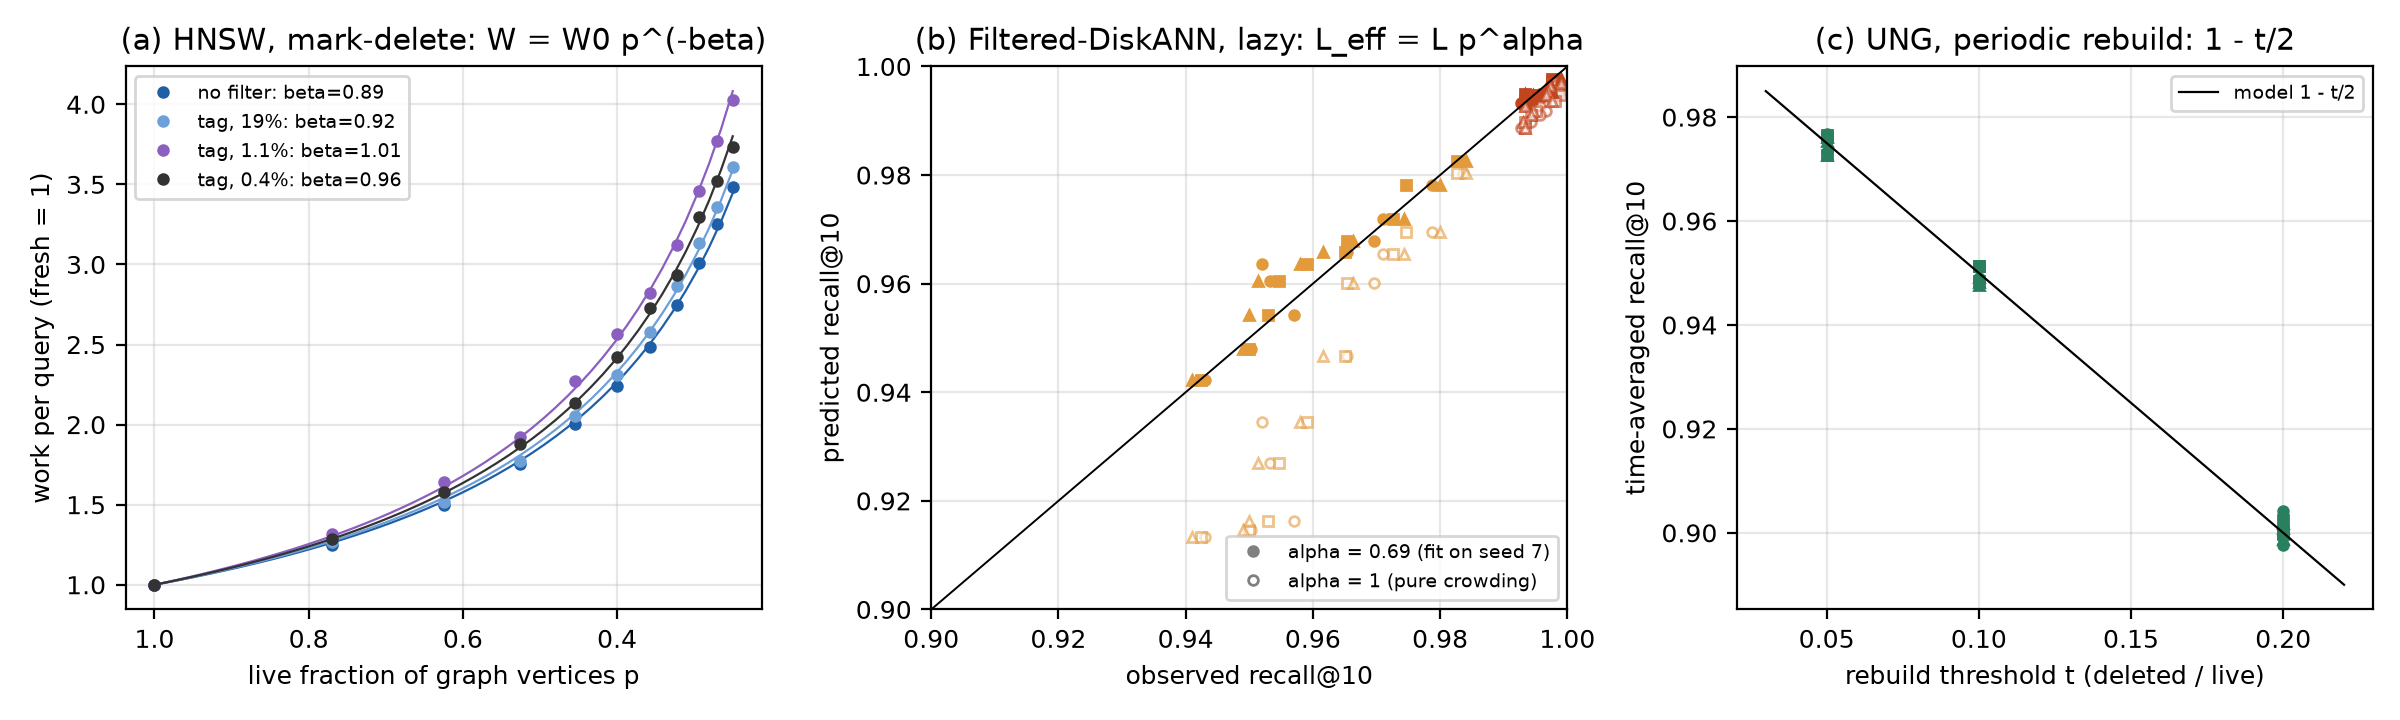
\includegraphics[width=\linewidth]{figures/fig_laws.png}
\caption{First-order laws. (a) HNSW, mark-delete, YFCC: work versus live fraction $p$ with fitted $p^{-\beta}$. (b) Filtered-DiskANN, lazy, SIFT, three seeds (markers), no filter (red) and 28\% filter (orange): predicted versus observed recall for $\alpha = 1$ (hollow) and $\alpha = 0.69$ fitted on one seed (filled). (c) UNG, SIFT, three seeds and three filters: time-averaged recall versus rebuild threshold.}
\label{fig:laws}
\end{figure}

\paragraph{First-order laws.} Each mechanism admits a one-parameter law (Figure~\ref{fig:laws}).

\emph{Traversal overhead (HNSW, mark-delete).} With $p$ the live fraction of graph vertices,
\begin{equation}
W(p) = W_0\,p^{-\beta}.
\end{equation}
Least-squares fits give $\beta = 0.89$ (no filter) to $1.01$--$1.02$ (1.1\% tag) on YFCC over three seeds with a mean relative error of 0.5--1.9\%, and $\beta = 0.87$--$0.94$ for latency on SIFT (1.3--3\%).

\emph{Candidate crowding (Filtered-DiskANN, lazy).} The degraded index behaves like a fresh index searched with a shorter list,
\begin{equation}
R(p) = R_{\text{fresh}}\!\left(L_{\text{eff}}\right),\qquad L_{\text{eff}} = L\,p^{\alpha},
\end{equation}
where $R_{\text{fresh}}(L)$ is measured once on a fresh index. Pure crowding ($\alpha=1$) captures the shape (correlation 0.97) but overestimates the loss by $1.6\times$. Probing the candidate list shows that the live share inside the list equals the live share of the graph (0.241 vs.\ 0.250), so the gap is not due to uneven placement of deleted vertices: deleted vertices occupy list slots but still serve as routes. The navigation term enters through $\alpha$: fitted on one seed ($\alpha=0.69$), it reduces the mean absolute error on two held-out seeds from 0.019 to 0.002--0.003 with a filter and from 0.003 to 0.001 without. On a run with a different list length ($L=64$) the same $\alpha$ halves the error (0.037 to 0.021) but the optimum there is $\alpha=0.80$: $\alpha$ depends on the search width.

\emph{Invisible insertions (static index, rebuild at $t$).} Between rebuilds a fraction of the collection growing from 0 to $t$ is invisible, so the time-averaged recall is
\begin{equation}
\bar R(t) = 1 - t/2,
\end{equation}
while the number of rebuilds per unit of churn is proportional to $1/t$. Over three seeds, three filters and $t \in \{0.05, 0.1, 0.2\}$ on SIFT the deviation is at most 0.004; on YFCC the mean recall at $t=0.2$ is 0.891--0.903 over three seeds and four filters.

\begin{figure}[t]
\centering
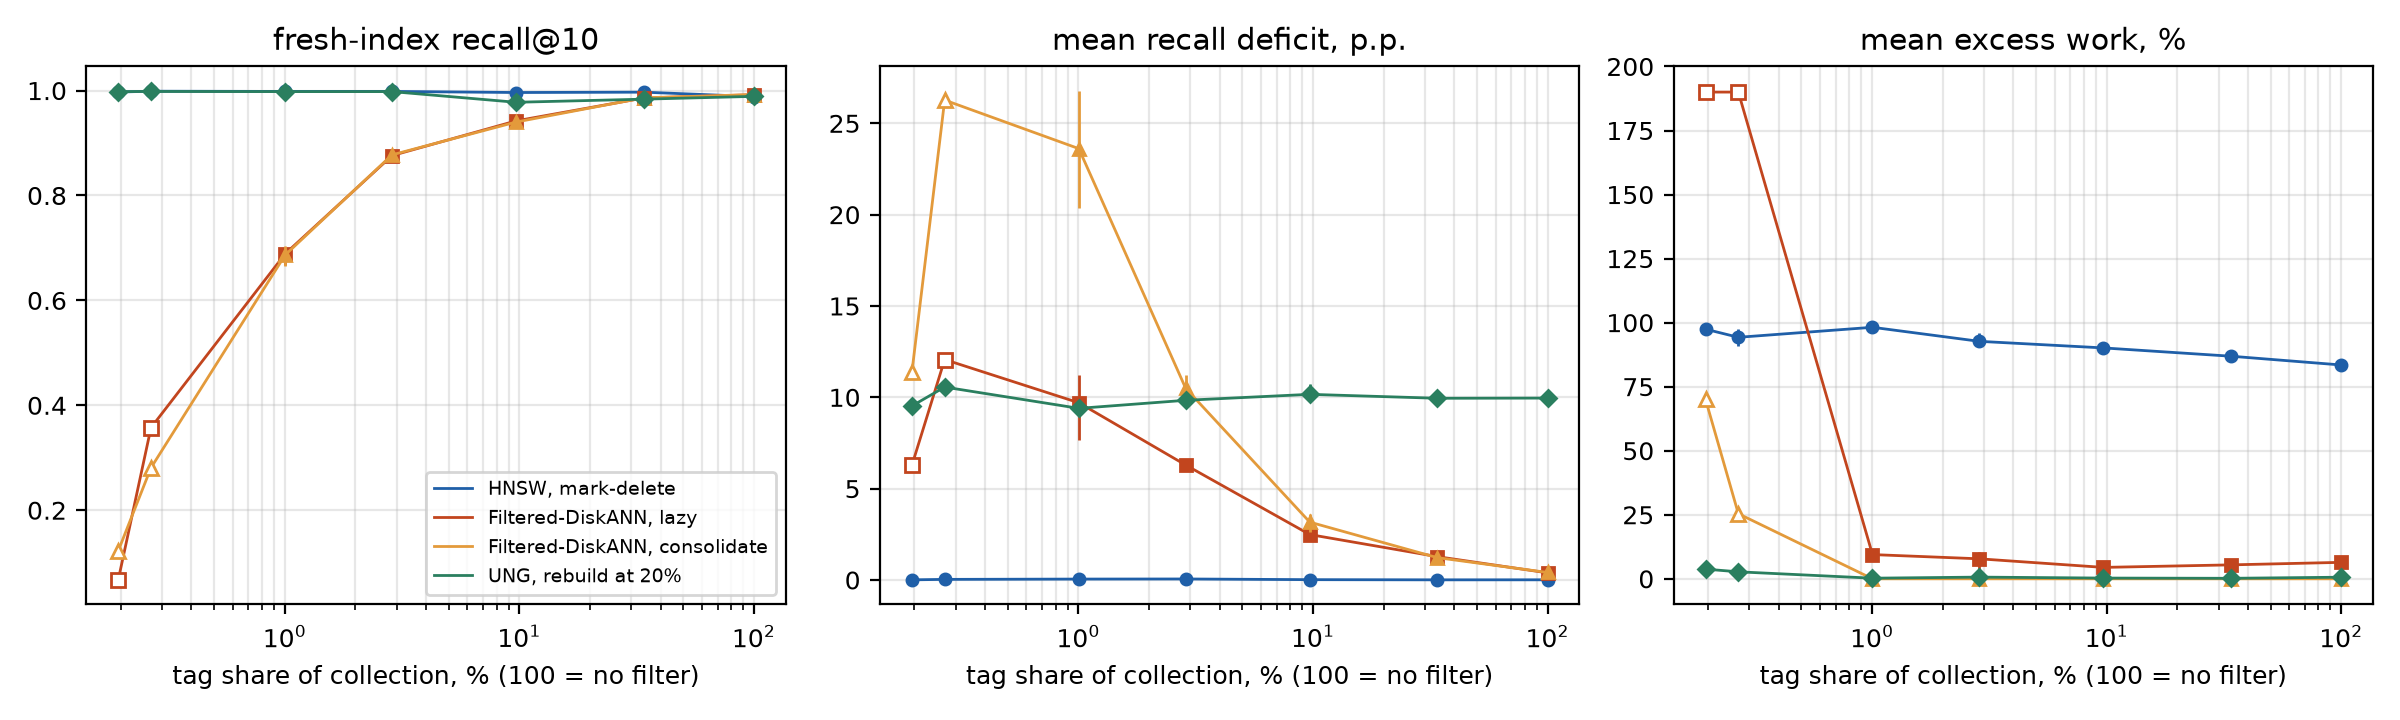
\includegraphics[width=\linewidth]{figures/fig_selectivity.png}
\caption{YFCC-10M, six tags from 34\% to 0.2\% of the collection, churn of 200k operations; mean over three seeds with min--max bars. Hollow markers: fresh-index recall below 0.5, where degradation metrics are meaningless.}
\label{fig:sel}
\end{figure}

\paragraph{Selectivity.} Figure~\ref{fig:sel} shows that selectivity matters only for one mechanism. Over three seeds, HNSW keeps recall 1.0 and its mean excess work (83--100\%) grows only mildly as the filter narrows; UNG loses 9.4--10.6 percentage points on average at every selectivity, as $1-t/2$ predicts. For Filtered-DiskANN the fresh-index recall already decreases as the filter narrows (0.99, 0.94, 0.88, 0.69 at 34, 10, 3, 1\%), the mean recall deficit under lazy deletion grows (0.4 p.p.\ without a filter; 1.3, 2.5, 6.3, 9.7 p.p.\ at 34, 10, 3, 1\%), and the number of operations until a 2-point loss shrinks from 160k--200k at 34\% to 80k--100k at 10\% and 40k--60k at 3--1\%. On tags covering 0.2--0.3\% the method fails already on a fresh index (recall 0.01--0.47). Selectivity alone does not explain this: tags of 0.39--0.40\% reached 0.86--0.91, and a measure of how strongly a tag clusters in the embedding space does not explain it either --- the failing tags are the most clustered. A second hardness factor is needed.

\paragraph{Category purge.} Deleting a whole category matters when the category occupies a region of space. With k-means labels on SIFT, purging a 7\% cluster made unfiltered recall of Filtered-DiskANN drop from 1.000 to 0.979 --- all of it on the 2.3\% of queries falling into the removed region, whose candidate lists fill with deleted vertices. Without consolidation the hole persisted (0.978 after 100k operations); the first consolidation restored 1.000. HNSW showed no such hole. With random labels the purge cost 1--2 points only.

\section{Implications for maintenance policy}

If degradation follows a known law, the maintenance threshold becomes the solution of an optimization problem rather than a constant. For a static index with rebuild cost $c$ per rebuild, churn rate $\lambda$ and value $v$ per unit of recall, the cost rate is $c\lambda/(t N) + v\,t/2$, minimized at $t^\ast = \sqrt{2c\lambda/(vN)}$. For HNSW the loss term is the extra work $W_0(p^{-\beta}-1)$, for Filtered-DiskANN the recall loss through $L_{\text{eff}}$, and the latter depends on filter selectivity. The industry constant of 20\% corresponds, in our measurements, to a mean recall of 0.90 for the static index and to 15--21\% extra work for HNSW at the moment maintenance is triggered. For two of the three mechanisms the degradation is explained by the simplest observable, the live fraction $p$; this agrees with the finding that structural repair signals do not beat scheduled repair at a matched budget for unfiltered graph indexes \cite{repair}, and suggests building maintenance policies on models of the operation stream rather than on graph-structure signals.

\section{Reproducibility pitfalls}
\label{sec:pitfalls}

None of the four methods built from the authors' instructions without changes to the build environment. ACORN crashes with a segmentation fault on the third call to \texttt{add} at $d=128$ (batches of 10k, 2k and 2k points; reproduced by a minimal program without any of our code), and each \texttt{add} allocates $O(N)$ locks, so a stream of insertions is impractical; we therefore excluded it from dynamic scenarios. In dynamic Filtered-DiskANN, filtered search by tag requires a label map that the dynamic index does not populate, and \texttt{insert\_point} silently requires each object's labels to be sorted: the label-intersection routine uses a two-pointer merge. With unsorted labels, objects were unreachable by any label except their first one --- 97--99\% of misses in our first YFCC runs --- and recall plateaued regardless of parameters. With labels uncorrelated to geometry, dynamic Filtered-DiskANN did not serve a 1.4\% filter even on a fresh index (recall $\approx$0.5\%): the start vertex of the label had almost no neighbors with the same label.

\section{Limitations}

Collections are 100k--400k objects; the laws must be checked at 1--10M. SIFT results, YFCC steady churn and the selectivity sweep have three seeds; category purge runs are single. The label vocabulary for YFCC is reduced to the queried tags, which changes the graph built by label-aware methods. One revision per method was studied. The laws are first-order: $\alpha$ depends on the search width, and the behavior of Filtered-DiskANN on rare tags is not explained by selectivity or tag clustering. Latency figures come from a single machine; work is reported as distance computations for that reason.

\section{Conclusion}

Degradation of filtered ANN indexes under churn is not a single phenomenon: it follows the maintenance mechanism --- traversal overhead, candidate crowding, invisible insertions --- and each mechanism admits a one-parameter law that fits held-out measurements closely. This supports replacing constant maintenance thresholds by thresholds derived from a model of the specific method and filter, and identifies rare-label filtered search in label-aware graphs as the part that first-order laws do not yet explain.

\paragraph{Artifact availability.} The protocol, method drivers, figure scripts and raw per-checkpoint results are available at \url{https://github.com/UKhAmster/filtered-ann-churn-public}.

\small
\begin{thebibliography}{99}
\bibitem{acorn} L.~Patel, P.~Kraft, C.~Guestrin, M.~Zaharia. ACORN: Performant and predicate-agnostic search over vector embeddings and structured data. \emph{Proc. ACM Manag. Data}, 2(3):1--27, 2024. doi:10.1145/3654923.
\bibitem{filtereddiskann} S.~Gollapudi, N.~Karia, V.~Sivashankar, R.~Krishnaswamy et al. Filtered-DiskANN: Graph algorithms for approximate nearest neighbor search with filters. In \emph{Proc. ACM Web Conference (WWW)}, pp.~3406--3416, 2023. doi:10.1145/3543507.3583552.
\bibitem{ung} Y.~Cai, J.~Shi, Y.~Chen, W.~Zheng. Navigating labels and vectors: A unified approach to filtered approximate nearest neighbor search. \emph{Proc. ACM Manag. Data}, 2(6):1--27, 2024. doi:10.1145/3698822.
\bibitem{hnsw} Yu.~A.~Malkov, D.~A.~Yashunin. Efficient and robust approximate nearest neighbor search using hierarchical navigable small world graphs. \emph{IEEE Trans. Pattern Anal. Mach. Intell.}, 42(4):824--836, 2020. doi:10.1109/TPAMI.2018.2889473.
\bibitem{qdrant} Qdrant issue \#7147. \url{https://github.com/qdrant/qdrant/issues/7147}, 2025.
\bibitem{vecbench} X.~Zhang, C.~Zhang, J.~Fan, G.~Li et al. VecBench: A controllable benchmark for filtered vector search. \emph{Proc. ACM Manag. Data}, 4(3):1--27, 2026. doi:10.1145/3802125.
\bibitem{annlib} Z.~Shen, Z.~Wan, J.~Su, Y.~Gu, Y.~Sun. ANNLib: A development framework for efficient approximate nearest neighbor search. arXiv:2607.17582, 2026.
\bibitem{freshdiskann} A.~Singh, S.~J.~Subramanya, R.~Krishnaswamy, H.~V.~Simhadri. FreshDiskANN: A fast and accurate graph-based ANN index for streaming similarity search. arXiv:2105.09613, 2021.
\bibitem{bigann23} H.~V.~Simhadri, M.~Aum\"uller, A.~Ingber, M.~Douze, G.~Williams, M.~Dobson Manohar et al. Results of the Big ANN: NeurIPS'23 competition. arXiv:2409.17424, 2024.
\bibitem{sift} H.~J\'egou, M.~Douze, C.~Schmid. Product quantization for nearest neighbor search. \emph{IEEE Trans. Pattern Anal. Mach. Intell.}, 33(1):117--128, 2011. doi:10.1109/TPAMI.2010.57.
\bibitem{yfcc} B.~Thomee, D.~A.~Shamma, G.~Friedland, B.~Elizalde et al. YFCC100M: The new data in multimedia research. \emph{Commun. ACM}, 59(2):64--73, 2016. doi:10.1145/2812802.
\bibitem{repair} M.~Mandarapu, S.~Kunkunuru. When to repair a graph ANN index: A matched-budget negative result, and the interpolated-baseline trap that hid it. arXiv:2607.00728, 2026.
\end{thebibliography}

\end{document}
